\section{The file directory}
\label{sec:dir}
A directory is a set of pairs, each pair consisting of a name (key) and an object (here: file). It
serves to retrieve objects by their name. If efficiency matters, the directory is organized as an
ordered set, ordered according to the keys. The most frequently used structures for ordered sets
are trees and hash tables. The latter have disadvantages when the size of the set is unknown,
particularly when its order of magnitude is unknown, and when deletions occur. The Oberon system
therefore uses a tree structure for its file directory, more specifically a B-tree, which was
developed especially for cases where not individual pairs, but only sets of pairs as a whole (placed on
a disk sector) can be accessed.

For a thorough study of B-trees we refer the reader to the literature \cite{Bayer, Comer}. Here it must
suffice to specify the B-tree's principal characteristics:
\begin{enumerate}
  \item In a B-tree of order $N$, each node (called page) contains $m$ elements (pairs), where
    $N \leq m \leq 2N$, except the root, where $0 \leq m \leq 2N$.
  \item A page with $m$ elements has either $0$ descendants, in which case it is called a leaf page, or
    $m + 1$ descendants.
  \item All leaf pages are on the same (bottom) level.
\end{enumerate}
From 3, it follows that the B-tree is a balanced tree. Its height, and with it the longest path's
length, has an upper bound of, roughly, $2 * \log{k}$, where $k$ is the number of elements and the
logarithm is taken to the base $N$ and rounded up to the next larger integer. Its minimal height is
$\log{k}$ taken to the base $2N$.

On each page, space must be available for $2N$ elements and for $2N + 1$ references to descendants.
Hence, $N$ is immediately determined by the size of a page and the size of elements.  In the case of
Oberon, names are limited to 32 characters (bytes), and the object is a reference to the associated file
(4 bytes). Each descendant pointer takes 4 bytes, and the page size is given by the sector size (1024)
minus the number of bytes needed to store $m$ (2 bytes).  Hence
\begin{verbatim}
  N = ((1024 - 2 - 4) DIV (32 + 4 + 4)) DIV 2 = 12
\end{verbatim}
A B-tree of height $h$ and order 12 may contain the following minimal and maximal number of elements:
\begin{table}
  \centering
  \begin{tabular}{c r r}
    height & minimum & maximum \\
    1      &       0 &      24 \\
    2      &      25 &     624 \\
    3      &     625 &   15624 \\
    4      &   15625 &  390624 \\
  \end{tabular}
\end{table}

It follows that the height of the B-tree will never be larger than 4, if the disk has a capacity of less
than about 400 MB, and assuming that each file occupies a single 1K sector. It is rarely larger than 3
in practice.

The definition of module \verb|FileDir| shows the available directory operations. Apart from the
procedures \verb|Search|, \verb|Insert|, \verb|Delete|, and \verb|Enumerate|, it contains some data
definitions, and it should be considered as the non-public part of the FS's interface.
\begin{verbatim}
DEFINITION FileDir;
  IMPORT SYSTEM, Kernel;

  CONST FnLength = 32; (*max length of file name*)
      SecTabSize = 64; (*no. of entries in primary table*)
       ExTabSize = 12;
      SectorSize = 1024;
       IndexSize = SectorSize DIV 4; (*no. of entries in index sector*)
      HeaderSize = 352;
      DirRootAdr = 29;
       DirPgSize = 24; (*max no. of elements on page*)

  TYPE DiskAdr = INT;
      FileName = ARRAY FnLength   OF CHAR;
    DataSector = ARRAY SectorSize OF BYTE;
   SectorTable = ARRAY SecTabSize OF DiskAdr;
ExtensionTable = ARRAY ExTabSize  OF DiskAdr;
  EntryHandler = PROC (name: FileName; sec: DiskAdr; VAR continue: BOOL);
    FileHeader = RECORD (*first page of each file on disk*)
                   mark: INT;
                   name: FileName;
                   aleng, bleng, date: INT;
                   ext: ExtensionTable;
                   sec: SectorTable
                 END ;
   IndexSector = RECORD (Kernel.Sector)
                   x: ARRAY IndexSize OF LONGINT;
                 END ;
      DirEntry = RECORD
                   name: FileName;
                   adr, p: DiskAdr
                 END ;
       DirPage = RECORD
                   mark: INT;
                   m: INT; (*no. of elements on page*)
                   p0: DiskAdr;
                   e: ARRAY DirPgSize OF DirEntry;
                 END ;

  PROC Search(name: FileName; VAR fad: DiskAdr);
  PROC Insert(name: FileName;     fad: DiskAdr);
  PROC Delete(name: FileName; VAR fad: DiskAdr);
  PROC Enumerate(prefix: ARRAY OF CHAR; proc: EntryHandler);
END FileDir.
\end{verbatim}

Procedures \verb|Search|, \verb|Insert|, and \verb|Delete| represent the typical operations performed on a directory.
Efficiency of the first operation is of primary importance. But the B-tree structure also guarantees
efficient insertion and deletion, although the code for these operations is complex. Procedure
\verb|Enumerate| is used to obtain excerpts of the directory. The programmer must guarantee that no
directory changes are performed by the parametric procedure of \verb|Enumerate|.

As in the presentation of module \verb|Files|, we first discuss a version that uses main storage rather
than a disk for the directory. This allows us to concentrate on the algorithms for handling the
directory, leaving out the additional complications due to the necessity to read pages (sectors) into
main store for selective updating and of restoring them onto disk. In particular, we point out the
definitions of the data types for B-tree nodes, called \verb|DirPage|, and elements, called
\verb|DirEntry|.  The component \verb|E.p| of an entry \verb|E| points to the page in which all elements
(with index \verb|k|) have keys \verb|E.p.e[k].name > E.name|. The pointer \verb|p.p0| points to a page
in which all elements have keys \verb|p.p0.e[k].name < p.e[0].name|. We can visualize these conditions
by Fig \ref{fig:b-tree}, where names have been replaced by integers as keys.
\begin{figure}
  \label{fig:b-tree}
  \centering
  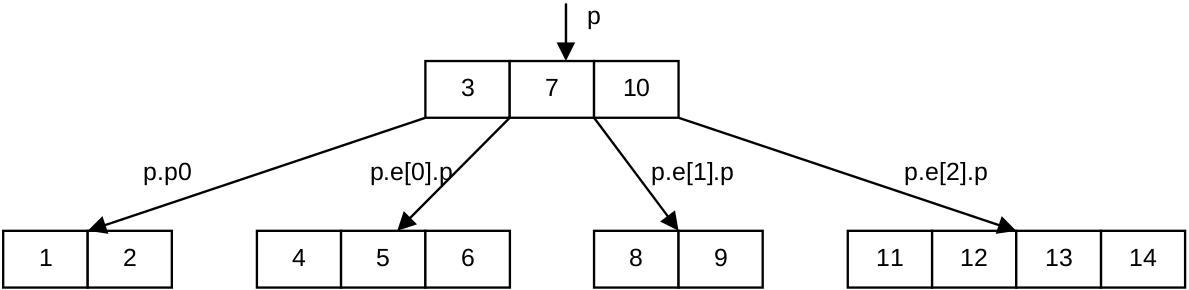
\includegraphics[width=\textwidth]{i/n}
  \caption{Example of a B-tree of order 2}
\end{figure}

Procedure \verb|Search| starts by inspecting the root page. It performs a binary search among its
elements, according to the following algorithm. Let \verb|e[0 ...  m-1]| be the ordered keys and
\verb|x| the search argument.
\begin{verbatim}
  L := 0; R := m;
  WHILE L < R DO
    i := (L+R) DIV 2;
    IF x <= e[i] THEN R := i ELSE L := i + 1 END
  END;
  IF (R < m) & (x = e[R]) THEN found END
\end{verbatim}

The invariant is
\[ e[L-1] < x \leq e[R] \]
If the desired element is not found, the search continues on the appropriate descendant page, if
there is one. Otherwise the element is not contained in the tree.

Procedures \verb|insert| and \verb|delete| use the same algorithm for searching an element within a
page.  However, they use recursion instead of iteration to proceed along the search path of pages. We
recall that the depth of recursion is at most 4. The reason for the use of recursion is that it
facilitates the formulation of structural changes, which are performed during the "unwinding" of
recursion, i.e. on the return path. First, the insertion point (respectively the position of the element
to be deleted) is searched, and then the element is inserted (deleted).

Upon insertion, the number of elements on the insertion page may become larger than $2N$, violating
B-tree condition 1. This situation is called page \emph{overflow}. The invariant must be reestablished
immediately. It could be achieved by moving one element from either end of the array \verb|e| onto a
neighbouring page. However, we choose not to do this, and instead to split the overflowing page into 2
pages immediately. The process of a \emph{page split} is visualized by Fig \ref{fig:page-split},
in which we distinguish between three cases, namely $R < N$, $R = N$, and $R > N$, where $R$ marks
the insertion point. $a$ denotes the overflowing, $b$ the new page, and $u$ the inserted element.
\begin{figure}
  \label{fig:page-split}
  \centering
  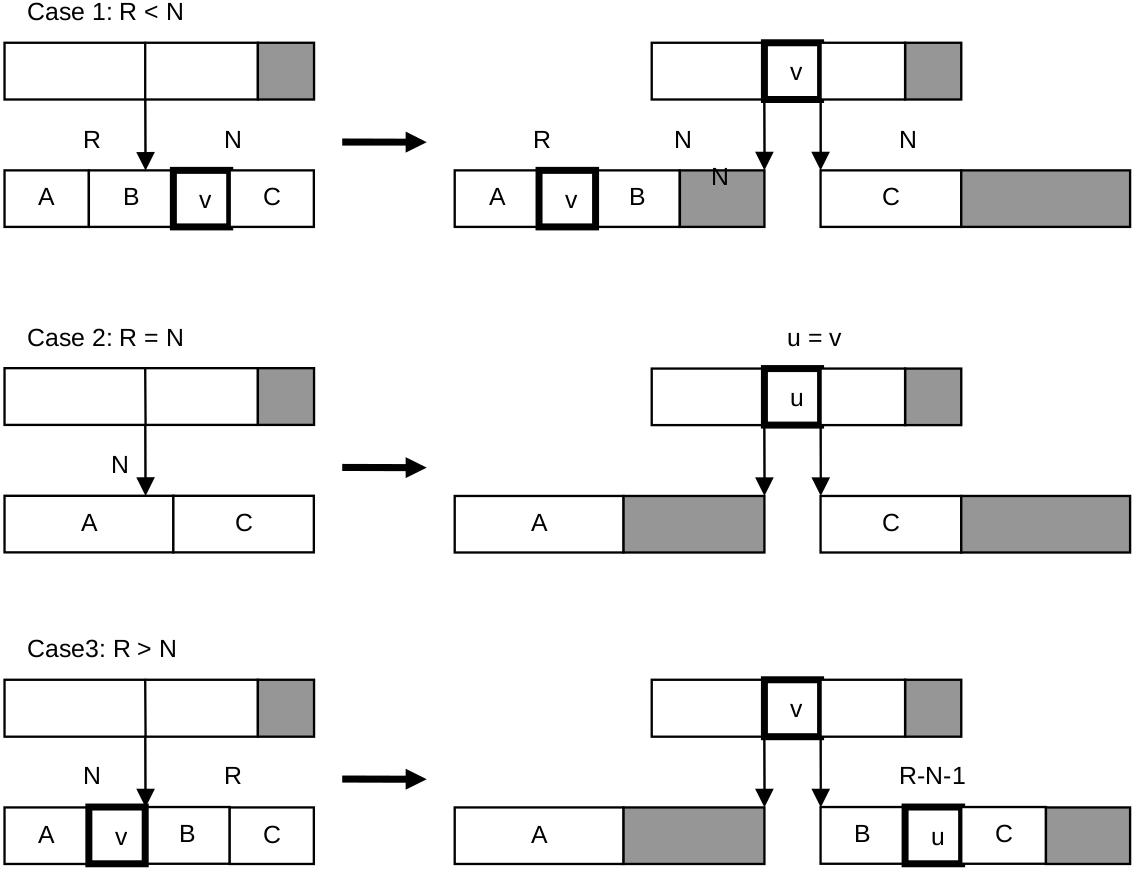
\includegraphics[width=.95\textwidth]{i/o}
  \caption{Page split when inserting element $u$}
\end{figure}

The $2N + 1$ elements ($2N$ from the full page $a$, plus the one element $u$ to be inserted) are equally
distributed onto pages $a$ and $b$. One element $v$ is pushed up in the tree. It must be inserted in the
ancestor page of $a$. Since that page obtains an additional descendant, it must also obtain an
additional element in order to maintain B-tree rule 2.

A page split may thus propagate, because the insertion of element $v$ in the ancestor page may
require a split once again. If the root page is full, it is split too, and the emerging element $v$ is
inserted in a new root page containing a single element. This is the only way in which the height
of a B-tree can increase.

When an element is to be deleted, it cannot simply be removed, if it resides on an internal page.
In this case, it is first replaced by another element, namely one of the 2 neighbouring elements
on a leaf page, i.e. the next smaller (or next larger) element, which is always on a leaf page. In
the presented solution, the replacing element is the largest on the left subtree (see procedure
\verb|del|). Hence, the actual deletion always occurs on a leaf page.

Upon deletion, the number of elements in a page may become less than $N$, violating invariant 1.
This event is called \emph{page underflow}. Since restructuring the tree is a relatively complicated
operation, we first try to reestablish the invariant by borrowing an element from a neighbouring
page. In fact, it is reasonable to borrow several elements, and thereby to decrease the likelihood
of an underflow on the same page upon further deletions. The number of elements that could be
taken from the neighbouring page $b$ is $b.m - N$. Hence we will borrow
\begin{verbatim}
  k = (b.m - N + 1) DIV 2
\end{verbatim}
elements. The process of page balancing then distributes the elements of the underflowing and its
neighbouring page equally to both pages (see procedure \verb|underflow|).

However, if (and only if) the neighbouring page has no elements to spare, the 2 pages can and must be
united. This action, called \emph{page merge}, places the $N-1$ elements from the underflowing page,
the $N$ elements from the neighbouring page, plus one element from the ancestor page onto a single page
of size $2N$. One element must be taken from the ancestor page, because that page loses one descendant
and invariant rule 2 must be maintained. The events of page balancing and merging are illustrated in
Fig \ref{fig:page-merge}.  $a$ is the underflowing page, $b$ its neighbouring page, and $c$ their
ancestor; $s$ is the position in the ancestor page of (the pointer to the) underflowing page $a$.  2
cases are distinguished, namely whether the underflowing page is the rightmost element ($s = c.m$)
or not (see procedure \verb|underflow|).
\begin{figure}
  \label{fig:page-merge}
  \centering
  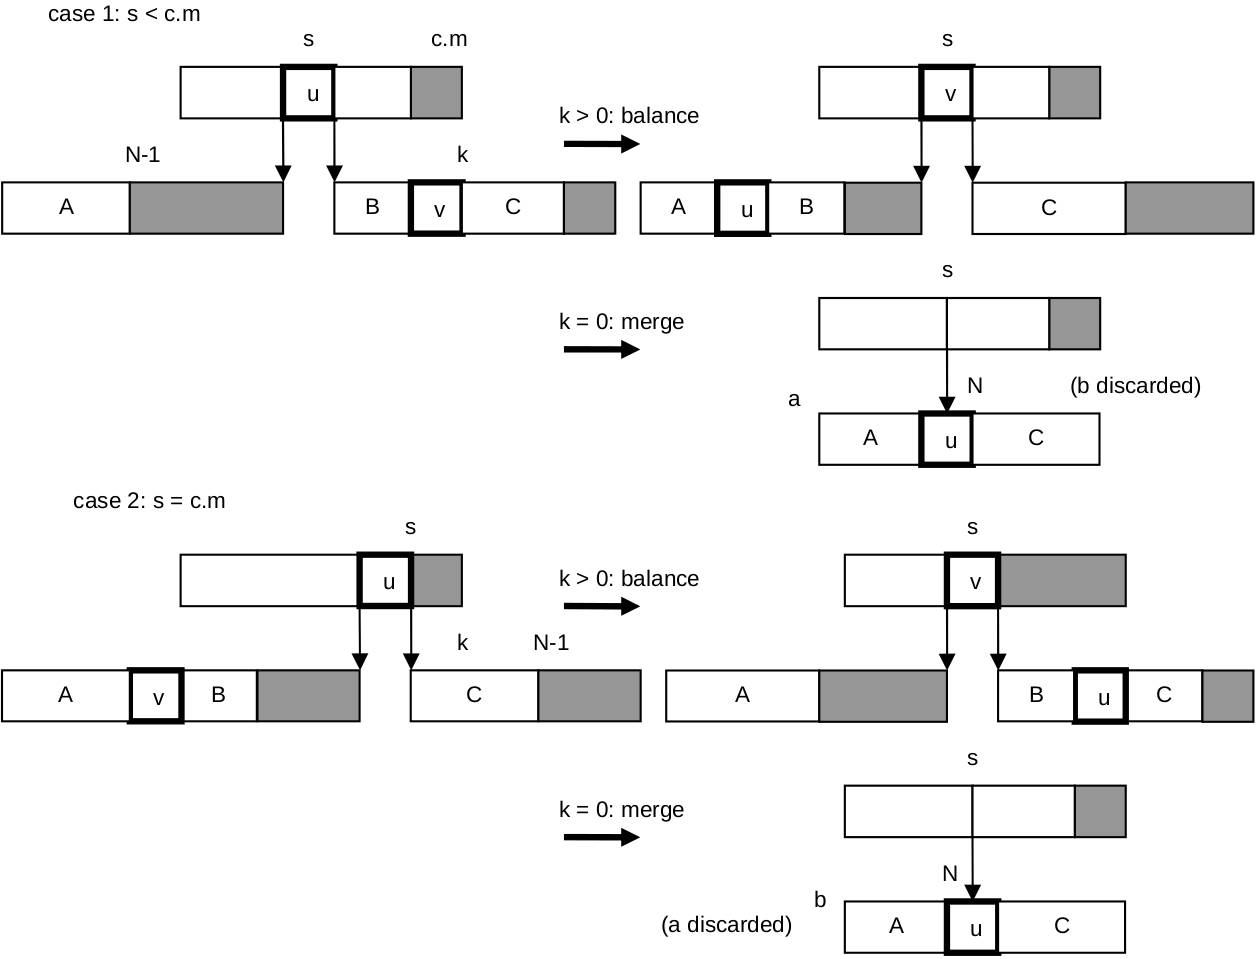
\includegraphics[width=.95\textwidth]{i/p}
  \caption{Page balancing and merging when deleting element}
\end{figure}

Similarly to the splitting process, merging may propagate, because the removal of an element
from the ancestor page may again cause an underflow, and perhaps a merge. The root page
underflows only if its last element is removed. This is the only way in which the B-tree's height
can decrease.
\begin{verbatim}
MODULE BTree;
  IMPORT Texts, Oberon;

  CONST N = 3;

  TYPE Page = POINTER TO PageRec;
      Entry = RECORD key, data: INT; p: Page END ;
    PageRec = RECORD m: INT; (*no. of entries on page*)
                p0: Page;
                e: ARRAY 2*N OF Entry
              END ;

  VAR root: Page; W: Texts.Writer;

  PROC search(x: INT; VAR p: Page; VAR k: INT);
    VAR i, L, R: INT; found: BOOL; a: Page;
  BEGIN a := root; found := FALSE;
    WHILE (a # NIL) & ~found DO
      L := 0; R := a.m; (*binary search*)
      WHILE L < R DO
        i := (L+R) DIV 2;
        IF x <= a.e[i].key THEN R := i ELSE L := i+1 END
      END ;
      IF (R < a.m) & (a.e[R].key = x) THEN found := TRUE
      ELSIF R = 0 THEN a := a.p0 ELSE a := a.e[R-1].p
      END
    END ;
    p := a; k := R
  END search;

  PROC insert(x: INT; a: Page; VAR h: BOOL; VAR v: Entry);
    (*a # NIL. Search key x in B-tree with root a;
      if found, increment counter. Otherwise insert new item with key x.
      If an entry is to be passed up, assign it to v.
      h := "tree has become higher"*)
    VAR i, L, R: INT; b: Page; u: Entry;
  BEGIN (*a # NIL & ~h*)
    L := 0; R := a.m; (*binary search*)
    WHILE L < R DO
      i := (L+R) DIV 2;
      IF x <= a.e[i].key THEN R := i ELSE L := i+1 END
    END ;
    IF (R < a.m) & (a.e[R].key = x) THEN (*found*) INC(a.e[R].data)
    ELSE (*item not on this page*)
      IF R = 0 THEN b := a.p0 ELSE b := a.e[R-1].p END ;
      IF b = NIL THEN (*not in tree, insert*)
        u.p := NIL; h := TRUE; u.key := x
      ELSE insert(x, b, h, u)
      END ;
      IF h THEN (*insert u to the left of a.e[R]*)
        IF a.m < 2*N THEN
          h := FALSE; i := a.m;
          WHILE i > R DO DEC(i); a.e[i+1] := a.e[i] END ;
          a.e[R] := u; INC(a.m)
        ELSE NEW(b); (*overflow; split a into a,b and assign the middle entry to v*)
          IF R < N THEN (*insert in left page a*)
            i := N-1; v := a.e[i];
            WHILE i > R DO DEC(i); a.e[i+1] := a.e[i] END ;
            a.e[R] := u; i := 0;
            WHILE i < N DO b.e[i] := a.e[i+N]; INC(i) END
          ELSE (*insert in right page b*)
            DEC(R, N); i := 0;
            IF R = 0 THEN v := u
            ELSE v := a.e[N];
              WHILE i < R-1 DO b.e[i] := a.e[i+N+1]; INC(i) END ;
              b.e[i] := u; INC(i)
            END ;
            WHILE i < N DO b.e[i] := a.e[i+N]; INC(i) END
          END ;
          a.m := N; b.m := N; b.p0 := v.p; v.p := b
        END
      END
    END
  END insert;

  PROC underflow(c, a: Page; s: INT; VAR h: BOOL);
    (*a = underflowing page, c = ancestor page,
      s = index of deleted entry in c*)
    VAR b: Page; i, k: INT;
  BEGIN (*h & (a.m = N-1) & (c.e[s-1].p = a) *)
    IF s < c.m THEN (*b := page to the right of a*)
      b := c.e[s].p; k := (b.m-N+1) DIV 2; (*k = nof items available on page b*)
      a.e[N-1] := c.e[s]; a.e[N-1].p := b.p0;
      IF k > 0 THEN (*balance by moving k-1 items from b to a*) i := 0;
        WHILE i < k-1 DO a.e[i+N] := b.e[i]; INC(i) END ;
        c.e[s] := b.e[k-1]; b.p0 := c.e[s].p;
        c.e[s].p := b; DEC(b.m, k); i := 0;
        WHILE i < b.m DO b.e[i] := b.e[i+k]; INC(i) END ;
        a.m := N-1+k; h := FALSE
      ELSE (*merge pages a and b, discard b*) i := 0;
        WHILE i < N DO a.e[i+N] := b.e[i]; INC(i) END ;
        i := s; DEC(c.m);
        WHILE i < c.m DO c.e[i] := c.e[i+1]; INC(i) END ;
        a.m := 2*N; h := c.m < N
      END
    ELSE (*b := page to the left of a*) DEC(s);
      IF s = 0 THEN b := c.p0 ELSE b := c.e[s-1].p END ;
      k := (b.m-N+1) DIV 2; (*k = nof items available on page b*)
      IF k > 0 THEN i := N-1;
        WHILE i > 0 DO DEC(i); a.e[i+k] := a.e[i] END ;
        i := k-1; a.e[i] := c.e[s]; a.e[i].p := a.p0;
        (*move k-1 items from b to a, one to c*) DEC(b.m, k);
        WHILE i > 0 DO DEC(i); a.e[i] := b.e[i+b.m+1] END ;
        c.e[s] := b.e[b.m]; a.p0 := c.e[s].p;
        c.e[s].p := a; a.m := N-1+k; h := FALSE
      ELSE (*merge pages a and b, discard a*)
        c.e[s].p := a.p0; b.e[N] := c.e[s]; i := 0;
        WHILE i < N-1 DO b.e[i+N+1] := a.e[i]; INC(i) END ;
        b.m := 2*N; DEC(c.m); h := c.m < N
      END
    END
  END underflow;

  PROC delete(x: INT; a: Page; VAR h: BOOL);
    (*search and delete key x in B-tree a; if a page underflow arises,
      balance with adjacent page or merge; h := "page a is undersize"*)
    VAR i, L, R: INT; q: Page;

    PROC del(p: Page; VAR h: BOOL);
      VAR k: INT; q: Page; (*global a, R*)
    BEGIN k := p.m-1; q := p.e[k].p;
      IF q # NIL THEN del(q, h);
        IF h THEN underflow(p, q, p.m, h) END
      ELSE p.e[k].p := a.e[R].p; a.e[R] := p.e[k];
        DEC(p.m); h := p.m < N
      END
    END del;
  BEGIN (*a # NIL*)
    L := 0; R := a.m; (*binary search*)
    WHILE L < R DO
      i := (L+R) DIV 2;
      IF x <= a.e[i].key THEN R := i ELSE L := i+1 END
    END ;
    IF R = 0 THEN q := a.p0 ELSE q := a.e[R-1].p END ;
    IF (R < a.m) & (a.e[R].key = x) THEN (*found*)
      IF q = NIL THEN (*a is leaf page*)
        DEC(a.m); h := a.m < N; i := R;
        WHILE i < a.m DO a.e[i] := a.e[i+1]; INC(i) END
      ELSE del(q, h);
        IF h THEN underflow(a, q, R, h) END
      END
    ELSE delete(x, q, h);
      IF h THEN underflow(a, q, R, h) END
    END
  END delete;

  PROC Search*(key: INT; VAR data: INT);
  BEGIN search(key, root, data)
  END Search;

  PROC Insert*(key: INT; VAR data: INT);
    VAR h: BOOL; u: Entry; q: Page;
  BEGIN h := FALSE; u.data := data; insert(key, root, h, u);
    IF h THEN (*insert new base page*)
      q := root; NEW(root);
      root.m := 1; root.p0 := q; root.e[0] := u
    END
  END Insert;

  PROC Delete*(key: INT);
    VAR h: BOOL;
  BEGIN h := FALSE; delete(key, root, h);
    IF h THEN (*base page size underflow*)
      IF root.m = 0 THEN root := root.p0 END
    END
  END Delete;

BEGIN NEW(root); root.m := 0
END BTree.
\end{verbatim}

The B-tree is also a highly appropriate structure for enumerating its elements, because during the
traversal of the tree each page is visited exactly once, and hence needs to be read (from disk)
exactly once too. The traversal is programmed by the procedure \verb|Enumerate| and uses recursion.
It calls the parametric procedure proc for each element of the tree. The type of proc specifies as
parameters the name and the (address of) the enumerated element. The third parameter continue is a
Boolean VAR-parameter. If the procedure sets it to FALSE, the process of enumeration will be aborted.

\verb|Enumerate| is used for obtaining listings of the names of registered files. For this purpose, the
actual procedure substituted for proc merely enters the given name in a text and ignores the address
(sector number) of the file, unless it requires special file information such as the file's size or
creation date.

The set of visited elements can be restricted by specifying a string which is to be a prefix to all
enumerated names. The least name with the specified prefix is directly searched and is the name (key)
of the first element enumerated. The process then proceeds up to the first element whose name does not
have the given prefix. Thereby, the process of obtaining all elements whose key has a given prefix
avoids traversal of the whole tree, resulting in a significant speedup. If the prefix is the empty
string, the entire tree is traversed.

The principle behind procedure \verb|Enumerate| is shown by the following sketch, where we abstract
from the B-tree structure and omit consideration of prefixes:
\begin{verbatim}
  PROC Enumerate(proc: PROC(name: FileName; adr: INT;
                            VAR continue: BOOL));
    VAR continue: BOOL; this: DirEntry;
  BEGIN continue := TRUE; this := FirstElement;
    WHILE continue & (this # NIL) DO
      proc(this.name, this.adr, continue);
      this := NextEntry(this)
    END
  END Enumerate
\end{verbatim}

From this sketch we may conclude that during the process of traversal the tree structure must not
change, because the function \verb|NextEntry| quite evidently relies on the structural information
stored in the elements of structure itself. Hence, the actions of the parametric procedure must not
affect the tree structure. Enumeration must not be used, for example, to delete a given set of files.
In order to prevent the misuse of the indispensible facility of element enumeration, the interface of
\verb|FileDir| is not available to users in general.

The handling of the directory stored on disk follows exactly the same algorithms. The accessed
pages are fetched from the disk as a whole (each page fits onto a single disk sector) and stored
in buffers of type \verb|DirPage|, from where individual elements can be accessed. In principle, these
buffers can be local to procedures insert and delete. A single buffer is allocated globally, namely
the one used by procedure Search. The reason for this exception is not only that iterative
searching requires one buffer only, but because procedure \verb|Files.Old| and in turn \verb|Search|
may be called when the processor is in the supervisor mode and hence uses the system- (instead of the
user-) stack, which is small and would not accommodate sector buffers.

Naturally, an updated page needs to be stored back onto disk. Omission of sector restoration is a
programming error that is very hard to diagnose, because some parts of the program are executed very
rarely, and hence the error may look sporadic and mistakenly be attributed to malfunctioning hardware.

Oberon's file directory represents a single, ordered set of name-file pairs. It is therefore also
called a \emph{flat directory}. Its internal tree structure is not visible to the outside. In contrast,
some file systems use a directory with a visible tree structure, notably UNIX. In a search, the name
(key) guides the search path; the name itself displays structure, in fact, it is a sequence of names
(usually separated by slashes or periods). The first name is then searched in the root directory,
whose descendants are not files but subdirectories. The process is repeated, until the last name
in the sequence has been used (and hopefully denotes a file).

Since the search path length in a tree increases with the logarithm of the number of elements,
any subdivision of the tree inherently decreases performance since $log(m + n) < log(m) + log (n)$
for any $m, n > 1$. It is justified only if there exist sets of elements with common properties. If
these property values are stored once, namely in the subdirectory referencing all elements with
common property values, instead of in every element, not only a gain in storage economy results,
but possibly also in accesses which depend on those properties. The common properties are typically
an owner's name, a password, and access rights (read or write protection), properties that primarily
have significance in a multi-user environment. Since Oberon was conceived explicitly as a single-user
system, there is little need for such facilities, and hence a flat directory offers the best
performance with a simple implementation.

Every directory operation starts with an access to the root page. An obvious measure for improving
efficiency is to store the root page "permanently" in main store. We have chosen not to do this for:
\begin{enumerate}
  \item If the hardware fails, or if the computer is switched off before the root page is copied to
    disk, the file directory will be inconsistent with severe consequences.
  \item The root page has to be treated differently from other pages, making the program more complex.
  \item Directory accesses do not dominate the computing process; hence, any improvement would hardly
    be noticeable in overall system performance. The payoff for the added complexity would be small.
  \item Procedure \verb|Init| is called upon system initialization in order to construct the sector
    reservation table. Therefore, this procedure (and the module) must be allowed to refer to the
    structure of a file's sector table(s), which is achieved by placing its definitions into the module
    \verb|FileDir| (instead of \verb|Files|). Unlike \verb|Enumerate|, \verb|Init| traverses the entire
    B-tree. The sector numbers of files delivered by \verb|TraverseDir| are entered into a buffer. When
    full, the entries are sorted, whereafter each file's head sector is read and the sectors indicated
    in its sector table are marked as reserved. The sorting speeds up the reading of the header sectors
    considerably. Nevertheless, the initialization of the sector reservation table clearly dominates
    the start-up time of the computer. For a file system with 10,000 files it takes in the order of 15s
    to record all files.
\end{enumerate}
